\documentclass[12pt]{article}
\usepackage{graphicx}
\usepackage{amssymb}
\usepackage{epstopdf}
\usepackage{amsmath}
\usepackage{multicol}
\usepackage{tcolorbox}
\usepackage{geometry}
\usepackage{enumitem}
\usepackage{fancyhdr}
\usepackage{pifont,amssymb} % for the symbols

\newlist{todolist}{itemize}{2}
\setlist[todolist]{label=$\square$}


\textwidth = 6.5 in
\textheight = 9 in
\oddsidemargin = 0.0 in
\evensidemargin = 0.0 in
\topmargin = -23pt
\headheight = 0.0 in
\headsep = 0.0 in
\parskip = 0.2in
\parindent = 0.0in
\pagestyle{fancy}
\pagenumbering{gobble}

\newtheorem{theorem}{Theorem}
\newtheorem{corollary}[theorem]{Corollary}
\newtheorem{definition}{Definition}
%\includegraphics [height=50mm, width=50mm]{PathInt.jpg}
\title{Title} 

\begin{document}
%INSTRUCTOR NOTES

 Name:
 \begin{center}\large{3.7 Implicit Differentiation}\end{center}

\begin{enumerate}
\item Find the points on the curve $x^2 + y^2 = 4$ where the slope of the tangent line is equal to $1$.

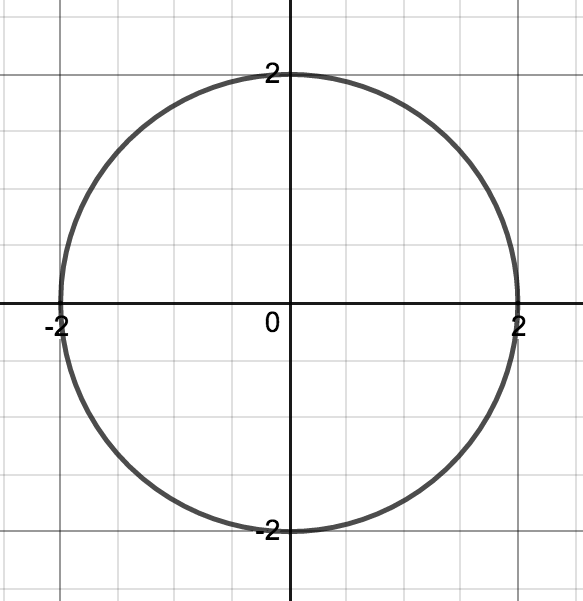
\includegraphics[width=2in]{3_7_implicit1.png}
\vfill

\item Find the equation of the tangent line to the curve $y^3 - xy + 6 = 0$ at $(7,2)$.
\vfill

\item The implicitly defined function $y^2 = x^3 - 3x + 1$ is shown below. Find the location of any points where the tangent line is horizontal.

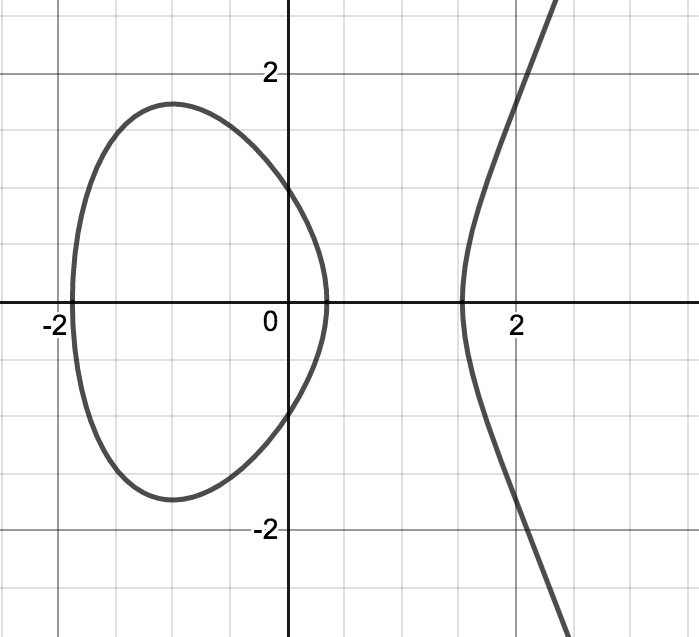
\includegraphics[width=2in]{3_7_implicit2.png}
\vfill

\newpage

$\hspace{10px}$ \\

\item At pressure P atmospheres, a certain fraction $f$ of a gas decomposes.The quantities $P$ and $f$ are related, for some positive $K$, by the equation

$$\frac{4f^2P}{1-f^2} = K$$

	\begin{enumerate}
	\item Find $\displaystyle \frac{df}{dP}$
	\vfill
	
	\item Show that $\frac{df}{dP} < 0$ always. What does this mean in practical terms?
	\vfill
	\end{enumerate}
	
\item Find $\displaystyle \frac{dy}{dx}$ for each of the following implicitly defined functions.

	\begin{enumerate}
	\item $\displaystyle yx^2 + 2y = y^2 + 1$
	\vfill
	
	\item $\displaystyle x^2y^2 + x\sin{(y)} = 4$
	\vfill
	
	\item $\displaystyle \frac{1}{e^{x^2 + y^2}} = e$	
	\vfill	
	\end{enumerate}
	

\end{enumerate}


\end{document} 
